\documentclass[polish,envcountsect,10pt]{beamer}
\usetheme{metropolis}
\usepackage[T1]{fontenc}
\usepackage{polski}
\usepackage{babel}
\usepackage{tikz}
\usepackage{xcolor}

\title{Triangulacja i diagramy Voronoi}
\author{Krzysztof Nasuta}
\date{Gdańsk, 2025}

\begin{document}

\frame{\titlepage}

\begin{frame}
  \frametitle{Definicje triangulacji w różnych dziedzinach matematyki}
  \begin{itemize}
    \item
      {
        \color<1>{violet}
        W geometrii triangulacja odnosi się do podziału płaszczyzny euklidesowej na trójkąty. W ogólności mówimy o \textbf{podziale przestrzeni euklidesowej na sympleksy}.
      }
    \item<2-> W teorii grafów występują dwie definicje triangulacji:
      \begin{itemize}
        \item
          {
            \color<2>{violet}
            \textbf{Tworzenie grafów maksymalnie planarnych}, czyli takich, do których nie można dodać żadnej krawędzi bez utraty własności planarnych. W grafie takim każda ścina jest trójkątem.
          }
        \item<3->
          {
            \color<3>{violet}
            \textbf{Dodawanie krawędzi do grafu w celu otrzymania grafu cięciwowego}, czyli takiego, w którym każdy cykl o długości czterech lub większej ma przekątną.
          }
      \end{itemize}
  \end{itemize}
\end{frame}

\begin{frame}
  \frametitle{Triangulacja w geometrii}
  \begin{definition}
    Sympleks to uogólnienie trójkąta i czworościanu na dowolne wymiary. Są to najprostsze możliwe obiekty geometryczne w danym wymiarze.
  \end{definition}

  \pause
  Dla przykładu:
  \begin{itemize}
    \item 0-wymiarowy sympleks to punkt,
    \item 1-wymiarowy sympleks to odcinek,
    \item 2-wymiarowy sympleks to trójkąt,
    \item 3-wymiarowy sympleks to czworościan,
  \end{itemize}
\end{frame}

\begin{frame}
  \frametitle{Triangulacja w geometrii}
  \begin{definition}
    Triangulacja to podział płaszczyzny euklidesowej na trójkąty. W ogólności mówi się o podziale przestrzeni euklidesowej na sympleksy odpowiedniego wymiaru.

    Zazwyczaj wymagane jest, aby krawędzie i wierzchołki sympleksów pokrywały się w całości z krawędziami i wierzchołkami innych sympleksów.
  \end{definition}
\end{frame}

\begin{frame}
  \frametitle{Triangulacja w geometrii - przykład dwuwymiarowy}
  \begin{center}
    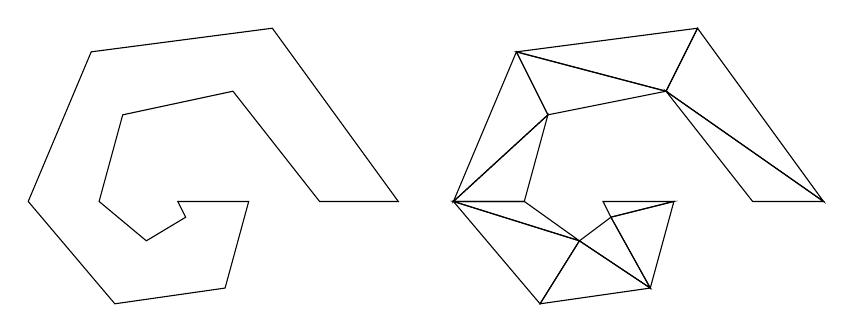
\begin{tikzpicture}
      \draw (1.3, 1.5) -- (1.6, 2.6) -- (3.0, 2.9) -- (4.1, 1.5) -- (5.1, 1.5) -- (3.5, 3.7) -- (1.2, 3.4) -- (0.4, 1.5) -- (1.5, 0.2) -- (2.9, 0.4) -- (3.2, 1.5) -- (2.3, 1.5) -- (2.4, 1.3) -- (1.9, 1.0) -- cycle;

      \pause
      \draw (7.8, 1.3) -- (7.4, 1.0) -- (8.3, 0.4) -- cycle;
      \draw (7.8, 1.3) -- (8.3, 0.4) -- (8.6, 1.5) -- cycle;
      \draw (7.8, 1.3) -- (8.6, 1.5) -- (7.7, 1.5) -- cycle;
      \draw (6.9, 0.2) -- (8.3, 0.4) -- (7.4, 1.0) -- cycle;
      \draw (6.9, 0.2) -- (7.4, 1.0) -- (5.8, 1.5) -- cycle;
      \draw (5.8, 1.5) -- (7.4, 1.0) -- (6.7, 1.5) -- cycle;
      \draw (5.8, 1.5) -- (6.7, 1.5) -- (7.0, 2.6) -- cycle;
      \draw (5.8, 1.5) -- (7.0, 2.6) -- (6.6, 3.4) -- cycle;
      \draw (7.0, 2.6) -- (8.5, 2.9) -- (6.6, 3.4) -- cycle;
      \draw (9.6, 1.5) -- (10.5, 1.5) -- (8.5, 2.9) -- cycle;
      \draw (8.9, 3.7) -- (6.6, 3.4) -- (8.5, 2.9) -- cycle;
      \draw (8.9, 3.7) -- (8.5, 2.9) -- (10.5, 1.5) -- cycle;
    \end{tikzpicture}
  \end{center}
\end{frame}

\begin{frame}
  \frametitle{Triangulacja w teorii grafów}
\end{frame}

\begin{frame}
  \frametitle{Triangulacja w teorii grafów}
\end{frame}

\begin{frame}
  \frametitle{Źródła}
  \begin{thebibliography}{4}
    \bibitem{1} \url{https://mathworld.wolfram.com/Triangulation.html}
    \bibitem{2} \url{https://en.wikipedia.org/wiki/Triangulation_(disambiguation)}
    \bibitem{3} \url{https://en.wikipedia.org/wiki/Planar_graph\#Maximal_planar_graphs}
    \bibitem{4} \url{https://en.wikipedia.org/wiki/Chordal_graph}
    \bibitem{5} \url{https://en.wikipedia.org/wiki/Simplex}
  \end{thebibliography}
\end{frame}

\end{document}
